\section{实验}

为了评估用于四旋翼控制的旋转误差度量,我们使用了以下三种情况。

\begin{enumerate}
  \item 方向改变。
  \item 具有大的初始偏航误差的轴对齐步骤。
  \item 对角线步骤。
\end{enumerate}

在最后两个实验中,我们还与基于欧拉角的旋转误差度量进行了比较,该度量是使用 Z-Y-X 约定定义的。
偏航 $\psi$、俯仰 $\theta$ 和横滚 $\phi$ 使用以下映射 $F(\psi, \theta, \phi)$ 定义旋转矩阵,其中 $c = \cos$ 并且 $s = \sin$。

\begin{align}
  F = \begin{pmatrix} c\psi c\theta & c\psi s\theta s\phi - c\phi s\psi & s\psi s \phi + c\psi c\phi s\theta \\
  c\theta s\psi & c\psi c\phi + s\psi s\theta s\phi & c\phi s\psi s\theta - c\psi s\phi \\
-s\theta & c\theta s\phi & c\theta c\phi \end{pmatrix}
\end{align}

然后使用 $F$ 的逆矩阵定义旋转误差度量,确保计算每个角度的最短角距离。

\begin{align}
  e_R^{\textbf{ZYX}}(R, \Rdes) = F^{-1}(R) \ominus F^{-1}(\Rdes)
\end{align}

\subsection{方向改变}

四旋翼飞机的任务是在原点以 $(0, -5, 0)$ 的速度和 $80^\circ$ 的初始横滚角开始后到达 $(0, 3, 0)$ 的目标位置。
这个初始条件被设计为诱导大于 $90^\circ$ 的初始横滚误差,以便突出大的角度误差下旋转误差度量反应的差异。

\begin{figure}
  \begin{center}
  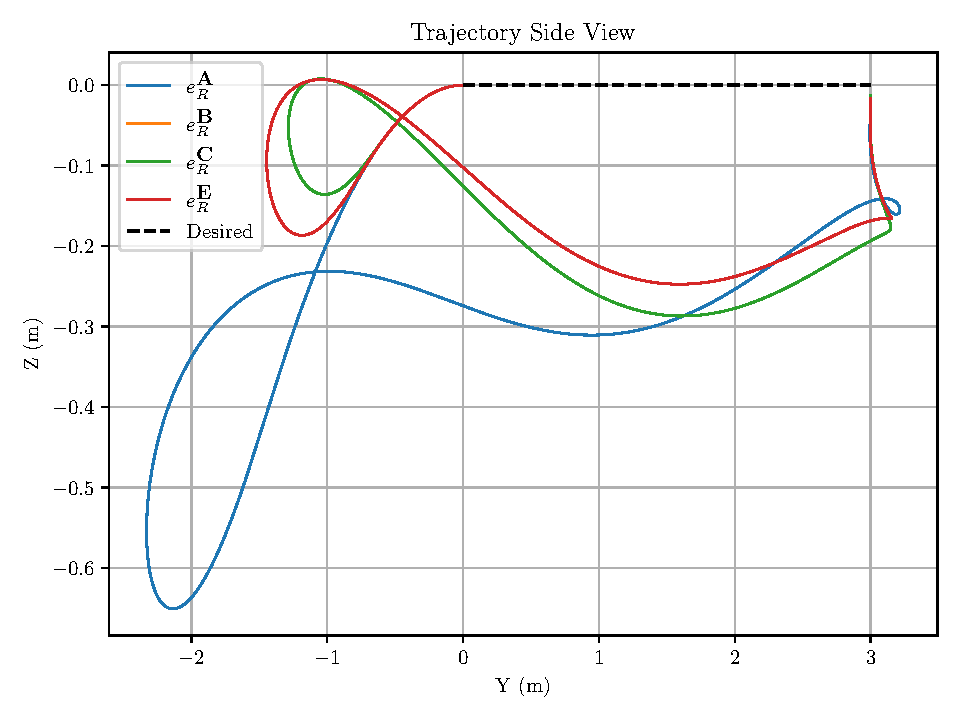
\includegraphics[width=8cm]{media/quickchange/sideview.pdf}
  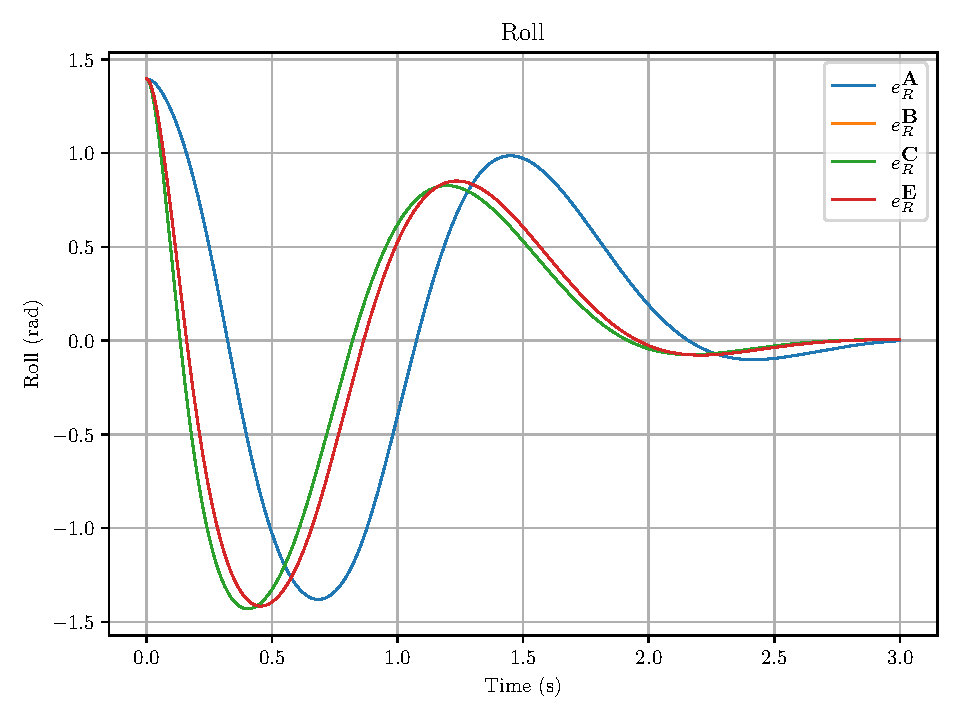
\includegraphics[width=8cm]{media/quickchange/Roll.pdf}
  \caption{在各种旋转误差度量的快速方向改变测试期间,跟踪轨迹(顶部)和横滚(底部)的侧视图。与角度正弦成比例的反应的度量,\textbf{A},其收敛速度远慢于与半角正弦,\textbf{B} 和 \textbf{E},或与角度,\textbf{C},成比例的反应的度量。由于轨迹位于 $YZ$ 平面中,\textbf{B} 和 \textbf{E} 执行相同的操作。}
  \label{fig:qc_side}
  \end{center}
\end{figure}

图~\ref{fig:qc_side} 显示了产生的侧视图和横滚轨迹。
这里需要注意的重要一点是,旋转误差度量 $e_R^{\textbf{A}}$,其反应与角度误差的正弦成比例,收敛速度比其它度量更慢。
该示例表明,当存在大的姿态误差时,导致反应与角度正弦成比例的度量可能会出现缓慢收敛。

\subsection{带有偏航误差的步骤}

在这个测试中,四旋翼飞机同时执行位置步骤和偏航步骤。
飞行器从原点开始,偏航角为 $90^\circ$,并以 $0^\circ$ 的偏航角移动到 $(0, 3, 0)$。

\begin{figure}
  \begin{center}
  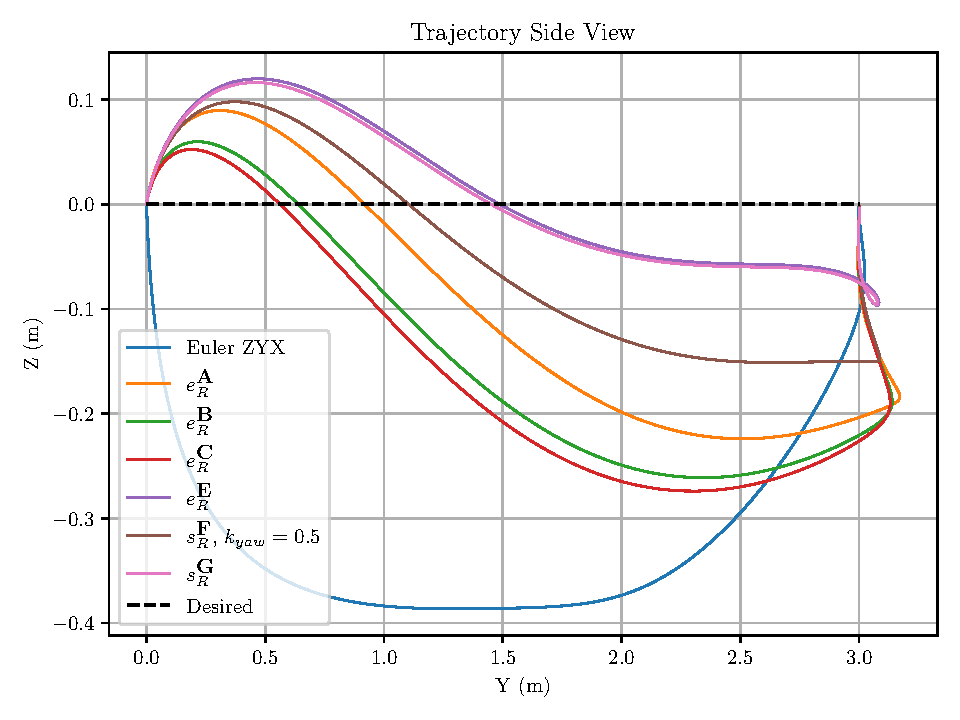
\includegraphics[width=8cm]{media/yawstep/sideview.pdf}
  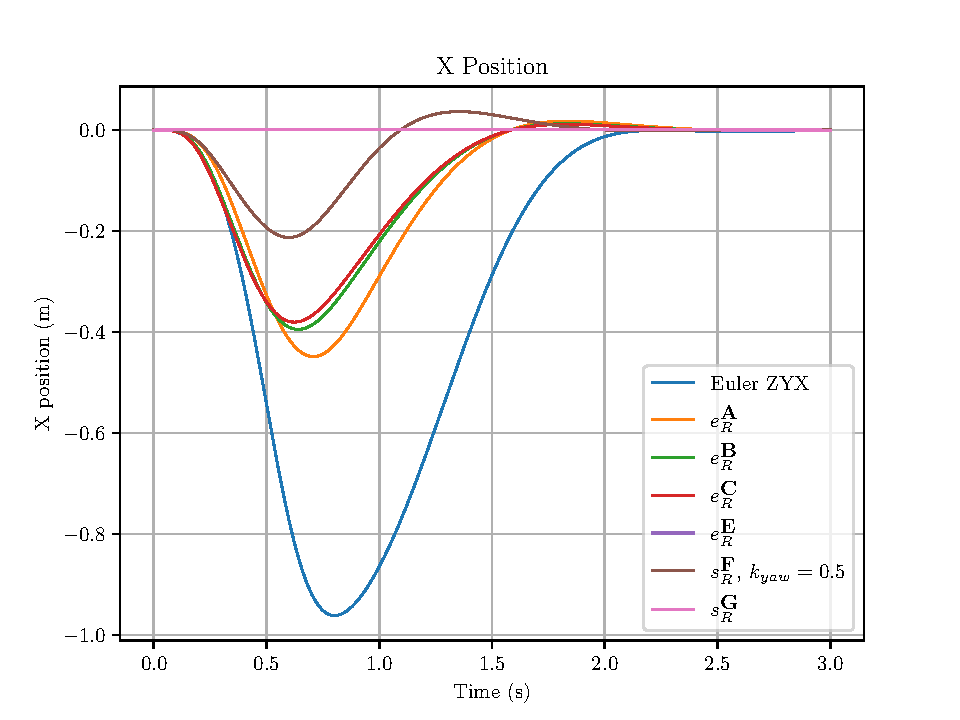
\includegraphics[width=8cm]{media/yawstep/X_Position.pdf}
  \caption{各种旋转误差度量下,在同时进行 $3$ m 位置步骤和 $90^\circ$ 偏航步骤期间,跟踪轨迹(顶部)和 $x$ 位置(底部)的侧视图。只有将推力向量从偏航中分解出来的度量,\textbf{E} 和 \textbf{G},才能保持期望的 $x$ 位置。}
  \label{fig:ys_side}
  \end{center}
\end{figure}

图~\ref{fig:ys_side} 显示了实验期间的侧视图和 $x$ 位置。
我们看到,使用全旋转误差的度量,导致轨迹不能保持期望的 $x$ 位置。
分解反应的度量,\textbf{E} 和 \textbf{G},保持了期望的 $x$ 位置。

\subsection{对角线步骤}

在这个测试中,我们表明,对于旋转误差度量,偏航误差不是必需的,因为旋转误差度量不会将推力矢量与偏航解耦,从而表现出次优性能。
四旋翼飞机被赋予一个从原点到 $(3, 3, 0)$ 的对角线步骤,在测试期间,期望的偏航为 $0^\circ$。

\begin{figure}
  \begin{center}
  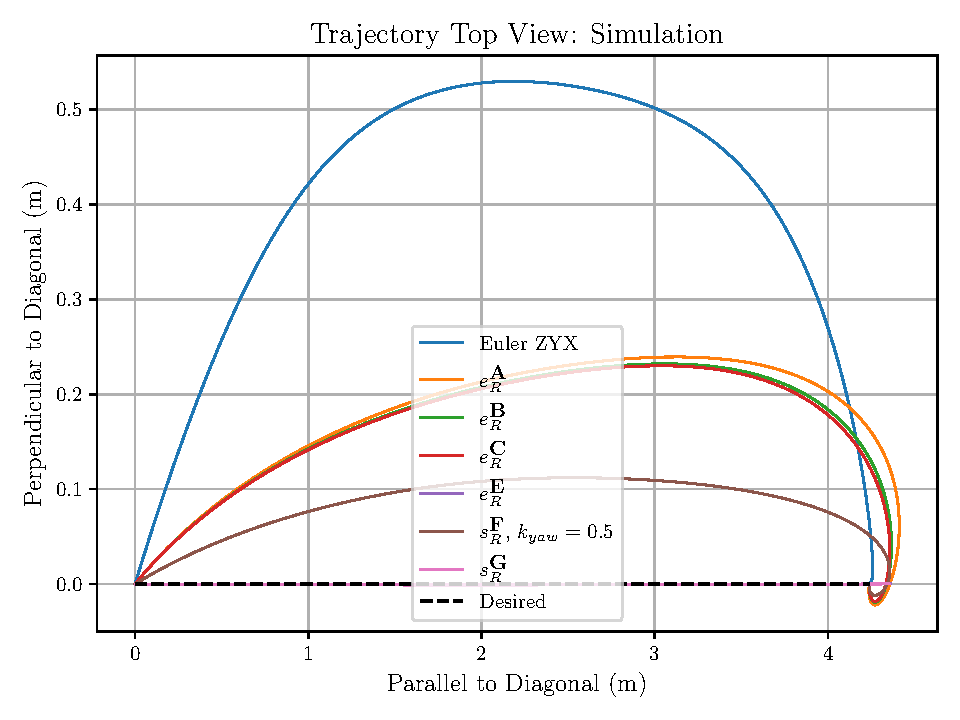
\includegraphics[width=8cm]{media/diagstep/topview.pdf}
  \caption{在从原点到 $(3, 3, 0)$ 的对角线步骤中,各种旋转误差度量的轨迹俯视图。只有将推力向量从偏航中分解出来的度量,\textbf{E} 和 \textbf{G},保持在直线的对角线路径上。}
  \label{fig:ds_top}
  \end{center}
\end{figure}

图~\ref{fig:ds_top} 显示了各种误差度量的实验过程中跟踪轨迹的俯视图。
使用全旋转误差的度量,\textbf{A},\textbf{B},\textbf{C} 和 \textbf{F},偏离了对角线路径。
这是因为在 $SO(3)$ 中,从幺元到导致飞行器以相同的偏航角的对角加速的最短路径,需要飞行器通过在对角以外的方向的加速方向。换句话说,投射到水平面上的推力向量并不指向期望位置的方向。

将误差分解为推力向量分量和偏航分量的度量,\textbf{E} 和 \textbf{G},沿着直线的对角线路径到达期望位置。
